%%**************************************************************
%% Vorlage fuer Bachelorarbeiten (o.ä.) der DHBW
%%
%% Autor: Tobias Dreher, Yves Fischer
%% Datum: 06.07.2011
%%
%% Autor: Michael Gruben
%% Datum: 15.05.2013
%%**************************************************************
\documentclass[%
	enabledeprecatedfontcommands,
	pdftex,
	oneside,		% Einseitiger Druck.
	12pt,			% Schriftgroesse
	parskip=half,	% Halbe Zeile Abstand zwischen Absätzen.
	headsepline,	% Linie nach Kopfzeile.
	footsepline,	% Linie vor Fusszeile.
	abstracton,	    % Abstract Überschriften
	ngerman,		% Translator
]{scrreprt}
%!TEX root = ../dokumentation.tex

%
% Nahezu alle Einstellungen koennen hier getaetigt werden
%



%Seitengroesse
\usepackage{fullpage}

%Zeilenumbruch und mehr
\usepackage[activate]{microtype}

% Zeichencodierung
\usepackage[utf8]{inputenc}
\usepackage[T1]{fontenc}

% Zeilenabstand
\usepackage[onehalfspacing]{setspace}

% Index-Erstellung
\usepackage{makeidx}

% Lokalisierung (neue deutsche Rechtschreibung)
\usepackage[ngerman]{babel}

% Anführungszeichen 
\usepackage[babel,german=quotes]{csquotes}
%\usepackage[style=swiss]{csquotes}


% Spezielle Tabellenform fuer Deckblatt
\usepackage{longtable}
\setlength{\tabcolsep}{10pt} %Abstand zwischen Spalten
\renewcommand{\arraystretch}{1.5} %Zeilenabstand

% Grafiken
\usepackage{graphicx}

% Mathematische Textsaetze
%\usepackage{amsmath}
%\usepackage{amssymb}

% Pakete um Textteile drehen zu können, oder eine Seite Querformat anzeigen kann.
%\usepackage{rotating}
%\usepackage{lscape}

% Farben
\usepackage{color}
\definecolor{LinkColor}{rgb}{0,0,0.2}
\definecolor{ListingBackground}{rgb}{0.92,0.92,0.92}

\newcommand{\pdftitel}{GamyTim Dokumentation}
\newcommand{\autor}{Vorname Nachname}
\newcommand{\arbeit}{Bachelorarbeit}

% Titel, Autor und Datum
\title{\titel}
\author{\autor}
\date{\datum}

% PDF Einstellungen
\usepackage[%
	pdftitle={\pdftitel},
	pdfauthor={\autor},
	pdfsubject={\arbeit},
	pdfcreator={pdflatex, LaTeX with KOMA-Script},
	pdfpagemode=UseOutlines, % Beim Oeffnen Inhaltsverzeichnis anzeigen
	pdfdisplaydoctitle=true, % Dokumenttitel statt Dateiname anzeigen.
	pdflang=de % Sprache des Dokuments.
]{hyperref} 

% (Farb-)einstellungen für die Links im PDF
\hypersetup{%
	colorlinks=true, % Aktivieren von farbigen Links im Dokument
	linkcolor=LinkColor, % Farbe festlegen
	citecolor=LinkColor,
	filecolor=LinkColor,
	menucolor=LinkColor,
	urlcolor=LinkColor,
	bookmarksnumbered=true % Überschriftsnummerierung im PDF Inhalt anzeigen.
}

% Literaturverweise nach Harvard (mit deutschem und)
\usepackage[dcucite]{harvard}
\renewcommand{\harvardand}{und}

% Verschiedene Schriftarten
%\usepackage{goudysans}
%\usepackage{lmodern}
%\usepackage{libertine}
\usepackage{palatino} 

% Hurenkinder und Schusterjungen verhindern
% http://projekte.dante.de/DanteFAQ/Silbentrennung
\clubpenalty=10000
\widowpenalty=10000
\displaywidowpenalty=10000

% Quellcode
\usepackage{listings}
\lstloadlanguages{Java}
\lstset{%
	language=PHP,		 	 % Sprache des Quellcodes
	%numbers=left,           % Zelennummern links
	stepnumber=1,            % Jede Zeile nummerieren.
	numbersep=5pt,           % 5pt Abstand zum Quellcode
	numberstyle=\tiny,       % Zeichengrösse 'tiny' für die Nummern.
	breaklines=true,         % Zeilen umbrechen wenn notwendig.
	breakautoindent=true,    % Nach dem Zeilenumbruch Zeile einrücken.
	postbreak=\space,        % Bei Leerzeichen umbrechen.
	tabsize=2,               % Tabulatorgrösse 2
	basicstyle=\ttfamily\footnotesize, % Nichtproportionale Schrift, klein für den Quellcode
	showspaces=false,        % Leerzeichen nicht anzeigen.
	showstringspaces=false,  % Leerzeichen auch in Strings ('') nicht anzeigen.
	extendedchars=true,      % Alle Zeichen vom Latin1 Zeichensatz anzeigen.
	captionpos=b,            % sets the caption-position to bottom
	backgroundcolor=\color{ListingBackground} % Hintergrundfarbe des Quellcodes setzen.
}
\usepackage{xcolor}

% Define JavaScript language for listings
\lstdefinelanguage{JavaScript}{
  keywords={break, case, catch, continue, debugger, default, delete, do, else, finally, for, function, if, in, instanceof, new, return, switch, this, throw, try, typeof, var, void, while, with, let, const, yield, import, export, class, extends, super},
  keywordstyle=\color{blue}\bfseries,
  ndkeywords={boolean, throw, implements, import, this},
  ndkeywordstyle=\color{darkgray}\bfseries,
  identifierstyle=\color{black},
  sensitive=false,
  comment=[l]{//},
  morecomment=[s]{/*}{*/},
  commentstyle=\color{gray}\ttfamily,
  stringstyle=\color{red}\ttfamily,
  morestring=[b]',
  morestring=[b]"
}

% General listings style
\lstset{
  language=JavaScript,
  backgroundcolor=\color{gray!10},
  basicstyle=\ttfamily\small,
  numbers=left,
  numberstyle=\tiny\color{gray},
  stepnumber=1,
  numbersep=8pt,
  showstringspaces=false,
  breaklines=true,
  frame=single,
  tabsize=2
}

% Glossar
\usepackage[
	nonumberlist, %keine Seitenzahlen anzeigen
	%acronym,      %ein Abkürzungsverzeichnis erstellen
	%section,     %im Inhaltsverzeichnis auf section-Ebene erscheinen
	toc,          %Einträge im Inhaltsverzeichnis
]{glossaries}

%Akronyme
\usepackage[printonlyused,footnote]{acronym}
\usepackage{adjustbox} % in die Präambel

% Fussnoten
\usepackage[perpage, hang, multiple, stable]{footmisc}

%Bildpfad
\graphicspath{{images/}}

%nur ein latex-Durchlauf für die Aktualisierung von Verzeichnissen nötig
\usepackage{bookmark}

%Gleitumgebungen (Bilder, Tabellen, usw\ldots) lassen sich mit H an genau der
% definierten Stelle platzieren
\usepackage{float}

% für die vertikale Platzierung von Text in Tabellen
\usepackage{array}

% für die Darstellung des Euro-Symbols
\usepackage[right]{eurosym}

% für textumflossene Grafiken
\usepackage{wrapfig}

% eine Kommentarumgebung "k" (Handhabe mit \begin{k}<Kommentartext>\end{k},
% Kommentare werden rot gedruckt). Wird \% vor excludecomment{k} entfernt,
% werden keine Kommentare mehr gedruckt.
\usepackage{comment}
\specialcomment{k}{\begingroup\color{red}}{\endgroup}
%\excludecomment{k}

\usepackage{longtable}
\usepackage{adjustbox}
\usepackage{caption} % optional, für schönere Tabellenbeschriftung
\usepackage{pdflscape} % in der Präambel

% Ab jetzt können auch Umlaute verwendet werden

%falls pdftitel = titel der Arbeit
\newcommand{\titel}{\pdftitel}
%bei unterschiedlichen Titeln
%\newcommand{\titel}{AudiTim Dokumentation}
%\newcommand{\martrikelnr}{}
\newcommand{\kurs}{INF2023AI}
\newcommand{\datumAbgabe}{September 2025}
\newcommand{\firma}{Aaron Reiber, Moritz Flaig}
%\newcommand{\firmenort}{Firmenort}
%\newcommand{\abgabeort}{Abgabeort}
%\newcommand{\abschluss}{Bachelor of Engineering}
%\newcommand{\studiengang}{Studienganges Vorderasiatische Archäologie}
\newcommand{\dhbw}{Heidenheim}
%\newcommand{\betreuer}{Luca Müller, Moritz Flaig}
%\newcommand{\gutachter}{Dr. Silvana Koch-Mehrin}
\newcommand{\zeitraum}{10 Wochen}
\newcommand{\arbeitsart}{\arbeit}

\makeglossaries
%!TEX root = ../dokumentation.tex

%
% vorher in Konsole folgendes aufrufen: 
%	makeglossaries makeglossaries dokumentation.acn && makeglossaries dokumentation.glo
%

%
% Glossareintraege --> referenz, name, beschreibung
% Aufruf mit \gls{...}
%
\newglossaryentry{Glossareintrag}{name={Glossareintrag},plural={Glossareinträge},description={Ein Glossar beschreibt verschiedenste Dinge in kurzen Worten}}


\begin{document}

	% Deckblatt
	\begin{spacing}{1}
		%!TEX root = ../dokumentation.tex

\begin{titlepage}
	\begin{longtable}{p{.4\textwidth} p{.4\textwidth}}
	  {
\includegraphics[height=2.6cm]{images/logo.png}} & 
	  {
\includegraphics[height=2.6cm]{images/dhbw.png}}
	\end{longtable}
	\enlargethispage{20mm}
	\begin{center}
	\vspace*{12mm}	{\LARGE\bf \titel }\\
    \vspace*{12mm} Verteilte-Systeme-Projekt\\
    \vspace*{3mm} des Studiengangs\\
    \vspace*{3mm} Allgemeine Informatik\\
    \vspace*{12mm} an der Dualen Hochschule Baden-Württemberg, Campus Heidenheim\\
	  %\vspace*{12mm}	{\large\bf \arbeit}\\
	  %\vspace*{12mm}	für die Prüfung zum\\
	  %\vspace*{3mm} 	{\bf \abschluss}\\
	  %\vspace*{12mm}	des \studiengang\\
	  %\vspace*{3mm} 	an der Dualen Hochschule Baden-Württemberg \dhbw\\
	  %\vspace*{12mm}	von\\
	  %\vspace*{3mm} 	{\large\bf \autor}\\
	  %\vspace*{12mm}	\datumAbgabe\\
	  \begin{center}
  \textit{Diese Dokumentation entstand im Rahmen des Verteilte-Systeme-Projekts 
  an der Dualen Hochschule Baden-Württemberg. 
  Sie beschreibt die Konzeption und Umsetzung von GamyTim, einem verteilten System zur sichergestellten Vergnügung, 
  dessen Ziel das hochverfügbare und sichere leaderboard-climben auf der GamyTim-Seite ist.}
\end{center}
	\end{center}
	\vfill
	\begin{spacing}{1.2}
	\begin{tabbing}
		mmmmmmmmmmmmmmmmmmmmmmmmmm     \= \kill
		\textbf{Bearbeitungszeitraum}  \>  \zeitraum\\
		\textbf{Kurs}  					\> \kurs\\
		\textbf{Gruppenmitglieder}      \>  \firma\\
		%\textbf{Gutachter}             \>  \gutachter
	\end{tabbing}
	\end{spacing}
\end{titlepage}

	\end{spacing}
	\newpage

	\renewcommand{\thepage}{\Roman{page}}
	\setcounter{page}{1}

	% Sperrvermerk
	%%!TEX root = ../dokumentation.tex

\thispagestyle{empty}
% Sperrvermerk direkt hinter Titelseite
\section*{Sperrvermerk}

\vspace*{2em}

Die vorliegende {\arbeitsart} mit dem Titel {\itshape \titel} ist mit einem Sperrvermerk versehen und wird ausschließlich zu Prüfungszwecken am Studiengang {\studiengang} der Dualen Hochschule Baden-Württemberg {\abgabeort} vorgelegt.
Jede Einsichtnahme und Veröffentlichung – auch von Teilen der Arbeit – bedarf der vorherigen Zustimmung durch die {\firma}.

	%\newpage
	
	% Erklärung
	%%!TEX root = ../dokumentation.tex

\thispagestyle{empty}

\section*{Erklärung}
% http://www.se.dhbw-mannheim.de/fileadmin/ms/wi/dl_swm/dhbw-ma-wi-organisation-bewertung-bachelorarbeit-v2-00.pdf
\vspace*{2em}

Ich erkläre hiermit ehrenwörtlich: \\
\begin{enumerate}
\item dass ich meine {\arbeitsart} mit dem Thema
{\itshape \titel } ohne fremde Hilfe angefertigt habe;
\item dass ich die Übernahme wörtlicher Zitate aus der Literatur sowie die Verwendung der Gedanken
anderer Autoren an den entsprechenden Stellen innerhalb der Arbeit gekennzeichnet habe;
\item dass ich meine {\arbeitsart} bei keiner anderen Prüfung vorgelegt habe;
\item dass die eingereichte elektronische Fassung exakt mit der eingereichten schriftlichen Fassung
übereinstimmt.
\end{enumerate}

Ich bin mir bewusst, dass eine falsche Erklärung rechtliche Folgen haben wird.

\vspace{3em}

\abgabeort, \datumAbgabe
\vspace{4em}

\autor

	%\newpage

	% Abstract
	%%!TEX root = ../dokumentation.tex

\pagestyle{empty}

\renewcommand{\abstractname}{Zusammenfassung}
\begin{abstract}
Ein Abstract ist eine prägnante Inhaltsangabe, ein Abriss ohne
Interpretation und Wertung einer wissenschaftlichen Arbeit. In DIN
1426 wird das (oder auch der) Abstract als Kurzreferat zur
Inhaltsangabe beschrieben.

\begin{description}
\item[Objektivität] soll sich jeder persönlichen Wertung enthalten
\item[Kürze] soll so kurz wie möglich sein
\item[Genauigkeit] soll genau die Inhalte und die Meinung der Originalarbeit wiedergeben
\end{description}

Üblicherweise müssen wissenschaftliche Artikel einen Abstract
enthalten, typischerweise von 100-150 Wörtern, ohne Bilder und
Literaturzitate und in einem Absatz.

Quelle \url{http://de.wikipedia.org/wiki/Abstract} Abgerufen 07.07.2011
\end{abstract}


\renewcommand{\abstractname}{Summary}
\begin{abstract}
An abstract is a brief summary of a research article, thesis, review,
conference proceeding or any in-depth analysis of a particular subject
or discipline, and is often used to help the reader quickly ascertain
the paper's purpose. When used, an abstract always appears at the
beginning of a manuscript, acting as the point-of-entry for any given
scientific paper or patent application. Abstracting and indexing
services for various academic disciplines are aimed at compiling a
body of literature for that particular subject.

The terms précis or synopsis are used in some publications to refer to
the same thing that other publications might call an "abstract". In
management reports, an executive summary usually contains more
information (and often more sensitive information) than the abstract
does.

Quelle: \url{http://en.wikipedia.org/wiki/Abstract_(summary)}

\end{abstract}

	%\newpage

	\pagestyle{plain}

	% Inhaltsverzeichnis
	\begin{spacing}{1.1}
		\setcounter{tocdepth}{1}
		%für die Anzeige von Unterkapiteln im Inhaltsverzeichnis
		%\setcounter{tocdepth}{2}
		\tableofcontents
	\end{spacing}
	\newpage

	\renewcommand{\thepage}{\arabic{page}}
	\setcounter{page}{1}
	
	% Inhalt
	\chapter{Einleitung}
\label{cha:einleitung}

Im Rahmen des Moduls „Verteilte Systeme“ haben wir gemeinsam ein Netzwerkspiel auf Basis des Klassikers „Achtung, Kurve!“ entwickelt. Ziel des Projekts war es, die Prinzipien verteilter Systeme praktisch umzusetzen und die Interaktion mehrerer Clients über einen zentralen Server zu ermöglichen.

\section{Projektüberblick}

Die Umsetzung erfolgte in Godot als Game Engine, ergänzt durch verschiedene Backend-Komponenten zur Verwaltung von Spielern, Lobbys und Spielzuständen. Dabei kamen unter anderem eine User-Datenbank, ein Redis-Server für schnelle Synchronisation, sowie ein Masterserver und ein Loadbalancer für die Organisation und Skalierung der Spielinstanzen zum Einsatz.

Die Architektur wurde so entworfen, dass sie eine saubere Trennung zwischen Frontend, Spiel-Logik und Backend-Systemen ermöglicht. Eine genauere Beschreibung der einzelnen Komponenten und deren Zusammenspiel erfolgt in den folgenden Kapiteln.

\section{Ziele und Motivation}

Dabei stand nicht nur der Spielspaß im Vordergrund, sondern insbesondere das praktische Verständnis von Konzepten wie:
Lastverteilung durch einen Loadbalancer, Zentrale Verwaltung von Lobbys und Spielzuständen über einen Masterserver, Persistente Datenspeicherung in Datenbanken, Skalierbarkeit durch die Nutzung mehrerer Game-Server und Redis für schnelle Synchronisation.

Die Motivation war also, ein praxisnahes Beispiel zu schaffen, bei dem die theoretischen Inhalte aus der Vorlesung in einem realen Projekt erlebbar werden. Durch die Umsetzung in Godot konnte zusätzlich die Anbindung einer Game Engine an ein verteiltes Backend erprobt werden.
	\chapter{Architektur}
\label{chap:architektur}

In diesem Kapitel wird die Architektur des Projekts beschrieben. 

\section{Überblick}
Die Gesamtarchitektur gliedert sich in mehrere Teilsysteme, die zusammenarbeiten, um ein stabiles Mehrspieler-Erlebnis zu gewährleisten. 
Das Spiel selbst läuft in Godot-Instanzen (Game-Server), die durch zentrale Backend-Komponenten verwaltet werden. 
Die Kommunikation erfolgt über klar definierte Schnittstellen zwischen Frontend, Loadbalancer, Masterserver, Datenbanken und Game-Servern. 
Ein schematischer Überblick ist in Abbildung~\ref{fig:architektur} dargestellt.

\begin{figure}[h!]
  \centering
  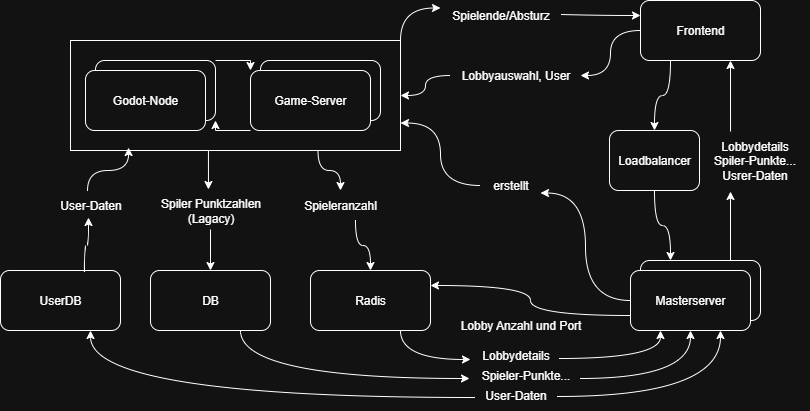
\includegraphics[width=0.95\linewidth]{../images/content.png}
  \caption{Architekturübersicht des Projekts}
  \label{fig:architektur}
\end{figure}


Bei der Planung der Architektur wurde stets darauf geachtet für den Benutzer die bestmögliche Erfahrung zu schaffen.
Hierfür wurde sich für WebSockets entschieden, um es dem Spieler zu ermöglichebn einfach im Browser zu spielen, ohne zusätzliche Software installieren zu müssen.
WebSockets bieten eine durchgehende Verbindung, bei der Client und Server jederzeit Daten senden können, was bei Echtzeit-Anwendungen wie Spielen die Verzögerung deutlich reduziert.
Vgl. hierzu auch:
(Alex Booker: *WebSockets vs HTTP: Which to choose for your project in 2024*, Ably, 13 min read \url{https://ably.com/topic/websockets-vs-http} (letzter Zugriff: 17.09.2025))


\section{Frontend}
Das Frontend stellt die Schnittstelle zum Spieler dar. 
Hier können Lobbys ausgewählt, Benutzer eingeloggt und Spieldetails angezeigt werden. 
Nach Spielende oder im Falle eines Absturzes liefert das Frontend entsprechendes Feedback an den Benutzer.
Dieses wurde in Angular umgesetzt und kommuniziert über HTTP und WebSockets mit dem Backend.
Angular wurde ausgewählt, da es eine moderne, komponentenbasierte Struktur bietet und die Entwicklung von Single-Page-Applications (SPAs) erleichtert. 
Außerdem war Angular bereits aus vorherigen Projekten bekannt, was die Einarbeitungszeit verkürzte.
\noindent
Vgl. hierzu auch:  
Sparkout Tech Solutions: \textit{Angular: Modern Web Application Development}, Medium, 28. Oktober 2023.  
URL: \url{https://sparkouttechsolutions.medium.com/angular-modern-web-application-development-ac2b3acdc878} (letzter Zugriff: 17.09.2025)


\section{Loadbalancer}
Der Loadbalancer verteilt eingehende Anfragen auf die verfügbaren Game-Server. 
Er sorgt dafür, dass neue Lobbys erstellt werden können und die Last gleichmäßig über mehrere Server verteilt wird. 
Dadurch wird die Skalierbarkeit des Systems gewährleistet.
Dieser wurde mit Nginx realisiert, da es eine bewährte Lösung für Lastverteilung darstellt. 
Es können beim Start der Container beliebig viele Masterserver-Instanzen angegeben werden. 
Dies geschieht unter dem Docker-Compose-Flag --scale masterserver=Anzahl. 

\section{Masterserver}
Der Masterserver (in Express) übernimmt die zentrale Verwaltung aller Lobbys und handhabt Informationen zu:
\begin{itemize}
  \item Anzahl und Ports der Lobbys,
  \item Spielern und deren Punkteständen,
  \item Metadaten wie Spielstatus und Benutzerinformationen.
\end{itemize}
Diese Daten werden sowohl an das Frontend als auch an die Game-Server weitergegeben.

\section{Game-Server und Godot}
Die eigentliche Spiellogik läuft in den Godot nodes, welche dann als HTML5 exportiert werden.
Das exportierte Spiel wird dann über die Game-Server dynamisch für den Client bereitgestellt. 
Jeder Game-Server repräsentiert eine Lobby und übernimmt die Synchronisation der Spielzustände zwischen den Spielern. 
Die Game-Server kommunizieren kontinuierlich über einen Redis-Cache mit dem Masterserver, um Daten wie Spieleranzahlen und Statusmeldungen zu übermitteln.
Die Punktestände sowie Userdaten werden in einer seperaten relationalen Datenbank gespeichert.

\section{Datenbanken}
Zur Verwaltung werden zwei Datenbanken eingesetzt:
\begin{itemize}
  \item \textbf{UserDB}: Speicherung von Benutzerinformationen wie Username und gehashtem Passwort in einer PostgreSQL-Datenbank. 
  \item \textbf{LeaderboardDB}: Speicherung von Spielerpunktzahlen und gespielten Spielen in einer PostgreSQL-Datenbank.
  \item \textbf{Redis}: Speicherung von Lobbydetails und temporären Statusdaten für schnelle Zugriffe und Synchronisation zwischen Masterserver und Game-Servern.
\end{itemize}

\section{Zusammenspiel}
Das Zusammenspiel der Komponenten erfolgt in folgenden Schritten:
\begin{enumerate}
  \item Ein Spieler wählt im Frontend eine Lobby aus oder erstellt eine neue.
  \item Der Loadbalancer leitet die Anfrage an den Masterserver weiter.
  \item Der Masterserver erstellt eine Lobby auf einem Game-Server und verwaltet alle relevanten Metadaten.
  \item Während des Spiels werden kontinuierlich Statusdaten (z.\,B. Punktestände, Spieleranzahlen) zwischen Game-Server, Redis und Masterserver ausgetauscht.
  \item Nach Spielende oder einem Absturz werden die Daten an das Frontend zurückgemeldet und gespeichert.
\end{enumerate}
	\chapter{Reflektion}
\section{Herausforderungen und Lösungen}
\subsection*{Synchronisation der Kollisionen}
\textbf{Problem:} Bei zwei offenen Tabs waren Crashes nicht synchron (bei einem Spieler „knapp vorbei“, beim anderen „voll drin“). \\
\textbf{Ursache:} Jeder Client prüfte lokal Kollisionen/Out-of-Bounds und hatte leicht unterschiedliche Arena-Bounds, FPS, RNG-Sequenzen.\\
\textbf{Lösung:} Nur der Host prüft Kollisionen auf seinem Spiel und beendet die Runde, bei einer Kollision. \\
Clients bekommen das Ergebnis vom Host mitgeteilt und beenden ihre Runde, egal ob sie lokal eine Kollision hatten oder nicht.\\
\textbf{Anmerkung:} Kann zwar zu Asynchronität führen, ist im Rahmen des Projekts aber vertretbar (Selbst große Spiele haben diese Synchronisationsprobleme).

\subsection*{Spieleranzahl-Übertragung}
\textbf{Problem:} Spieleranzahl wurde nicht im Frontend oder nur beim festgelegten "Dev"-Server angezeigt.\\
\textbf{Ursache:} Der GameServer wusste nicht auf welchem Port er läuft und konnte somit nicht die Spieleranzahl an den Masterserver übertragen. Somit hat er die Spielerzahl immer nur für den festgelegten Port des "Dev"-Servers übertragen.\\
\textbf{Lösung:} Der wichtigste Aspekt war die Differenzierung zwischen Internal- und Public-Port. Intern kann immer auf dem "Dev"-Port (standard) kommuniziert werden der Public-Port musste jedoch vom Masterserver identifiziert und für die spielerzahl festegelegt werden. \\

\subsection*{Username-Übergabe an Godot}
\textbf{Problem:} Der Username wird im Frontend erstellt und in der Datenbank gespeichert, jedoch nicht direkt an Godot übergeben.\\
\textbf{Ursache:} Godot hat keinen direkten Zugriff auf die Datenbank und fragt bei der Authentifizierung mit dem Token nur den Login-Service ab.\\
\textbf{Lösung:} Der Username wird in der URL (so wie der Auth-Token) als Query-Parameter übergeben und von Godot ausgelesen.\\
\textbf{Anmerkung:} Dabei war das ganze vorerst nicht trivial. Das Auslesen und Weiterverarbeiten von Query-Parametern in der Engine musste zunächst manuell implementiert werden.


\section{Mögliche Alternativen}
\subsection*{Synchronisation der Kollisionen}
Anstatt ein großes Spielfeld mit "auf Pixeln" basierter Kollisionsprüfung zu verwenden, könnte man das Spielfeld in ein Raster aufteilen und die Positionen der Spieler auf die Rasterzellen beschränken.
-> Räumliche Indexierung (z. B. Grid/Quadtree) für die Trails und Köpfe der einzelnen Spieler.

\subsection*{Spawnpositionen}
Derzeit werden die Spawnpositionen der Spieler zufällig gewählt, was zu unfairen Startbedingungen führen kann (z. B. wenn Spieler zu nah beieinander spawnen oder sehr nah am Rand). 
Dies war jedoch eine bewusste Designentscheidung, um das Spiel dynamisch und spannend zu gestalten.
Als Alternative wären auch vordefinierte Spawnpunkte denkbar, die strategisch über das Spielfeld verteilt sind, welche zu einem faireren Start führen würden, auf Kosten der Spannung.  

\section{Lessons Learned}
\subsection*{Login mit PostgreSQL und JWT}
Die Implementierung eines des Logins mit PostgreSQL und JWT war mit erstaunlich wenig Einarbeitungszeit verbunden und hat sich als sehr effektiv erwiesen.
Die Gruppenmitglieder hatten zuvor hiermit noch nicht gearbeitet, sind aber positiv überrascht und werden diese Erkenntnis in zukünftigen Projekten anwenden.

\subsection*{Datencache mit Redis}
Auch hiermit hatten die Gruppenmitglieder zuvor noch nicht gearbeitet und waren positiv überrascht, wie einfach und effektiv die Implementierung eines Datencaches mit Redis war.

\subsection*{Godot Engine}
Die Godot Engine war für alle Gruppenmitglieder neu und die Einarbeitung hat verhältnismäsig viel Zeit (im Vergleich zu anderen neu-erlernten Technologien) in Anspruch genommen.
Auch die Arbeit nach der Einarbeitung war teilweise etwas umständlich und ging eher schleppend voran. 
Die Komplexität und Größe des Codes und Architektur in Godot wurde zu Beginn stark unterschätzt.
	\chapter{UI (optionale Erläuterung)}
\section{Frontend-Lobby}
\label{chap:frontend}

Die \textit{Lobby} bildet den Einstiegspunkt für die Spieler und ist der zentrale Bestandteil des Frontends. 
Sie wurde mit dem Framework \textbf{Angular} umgesetzt und mit \textbf{Bootstrap} für ein modernes, responsives Design gestaltet. 
Die in Abbildung~\ref{fig:frontend_lobby} dargestellte Oberfläche ermöglicht den Login, die Serverauswahl sowie die Anzeige von Spielstatistiken.

\begin{figure}[h!]
  \centering
  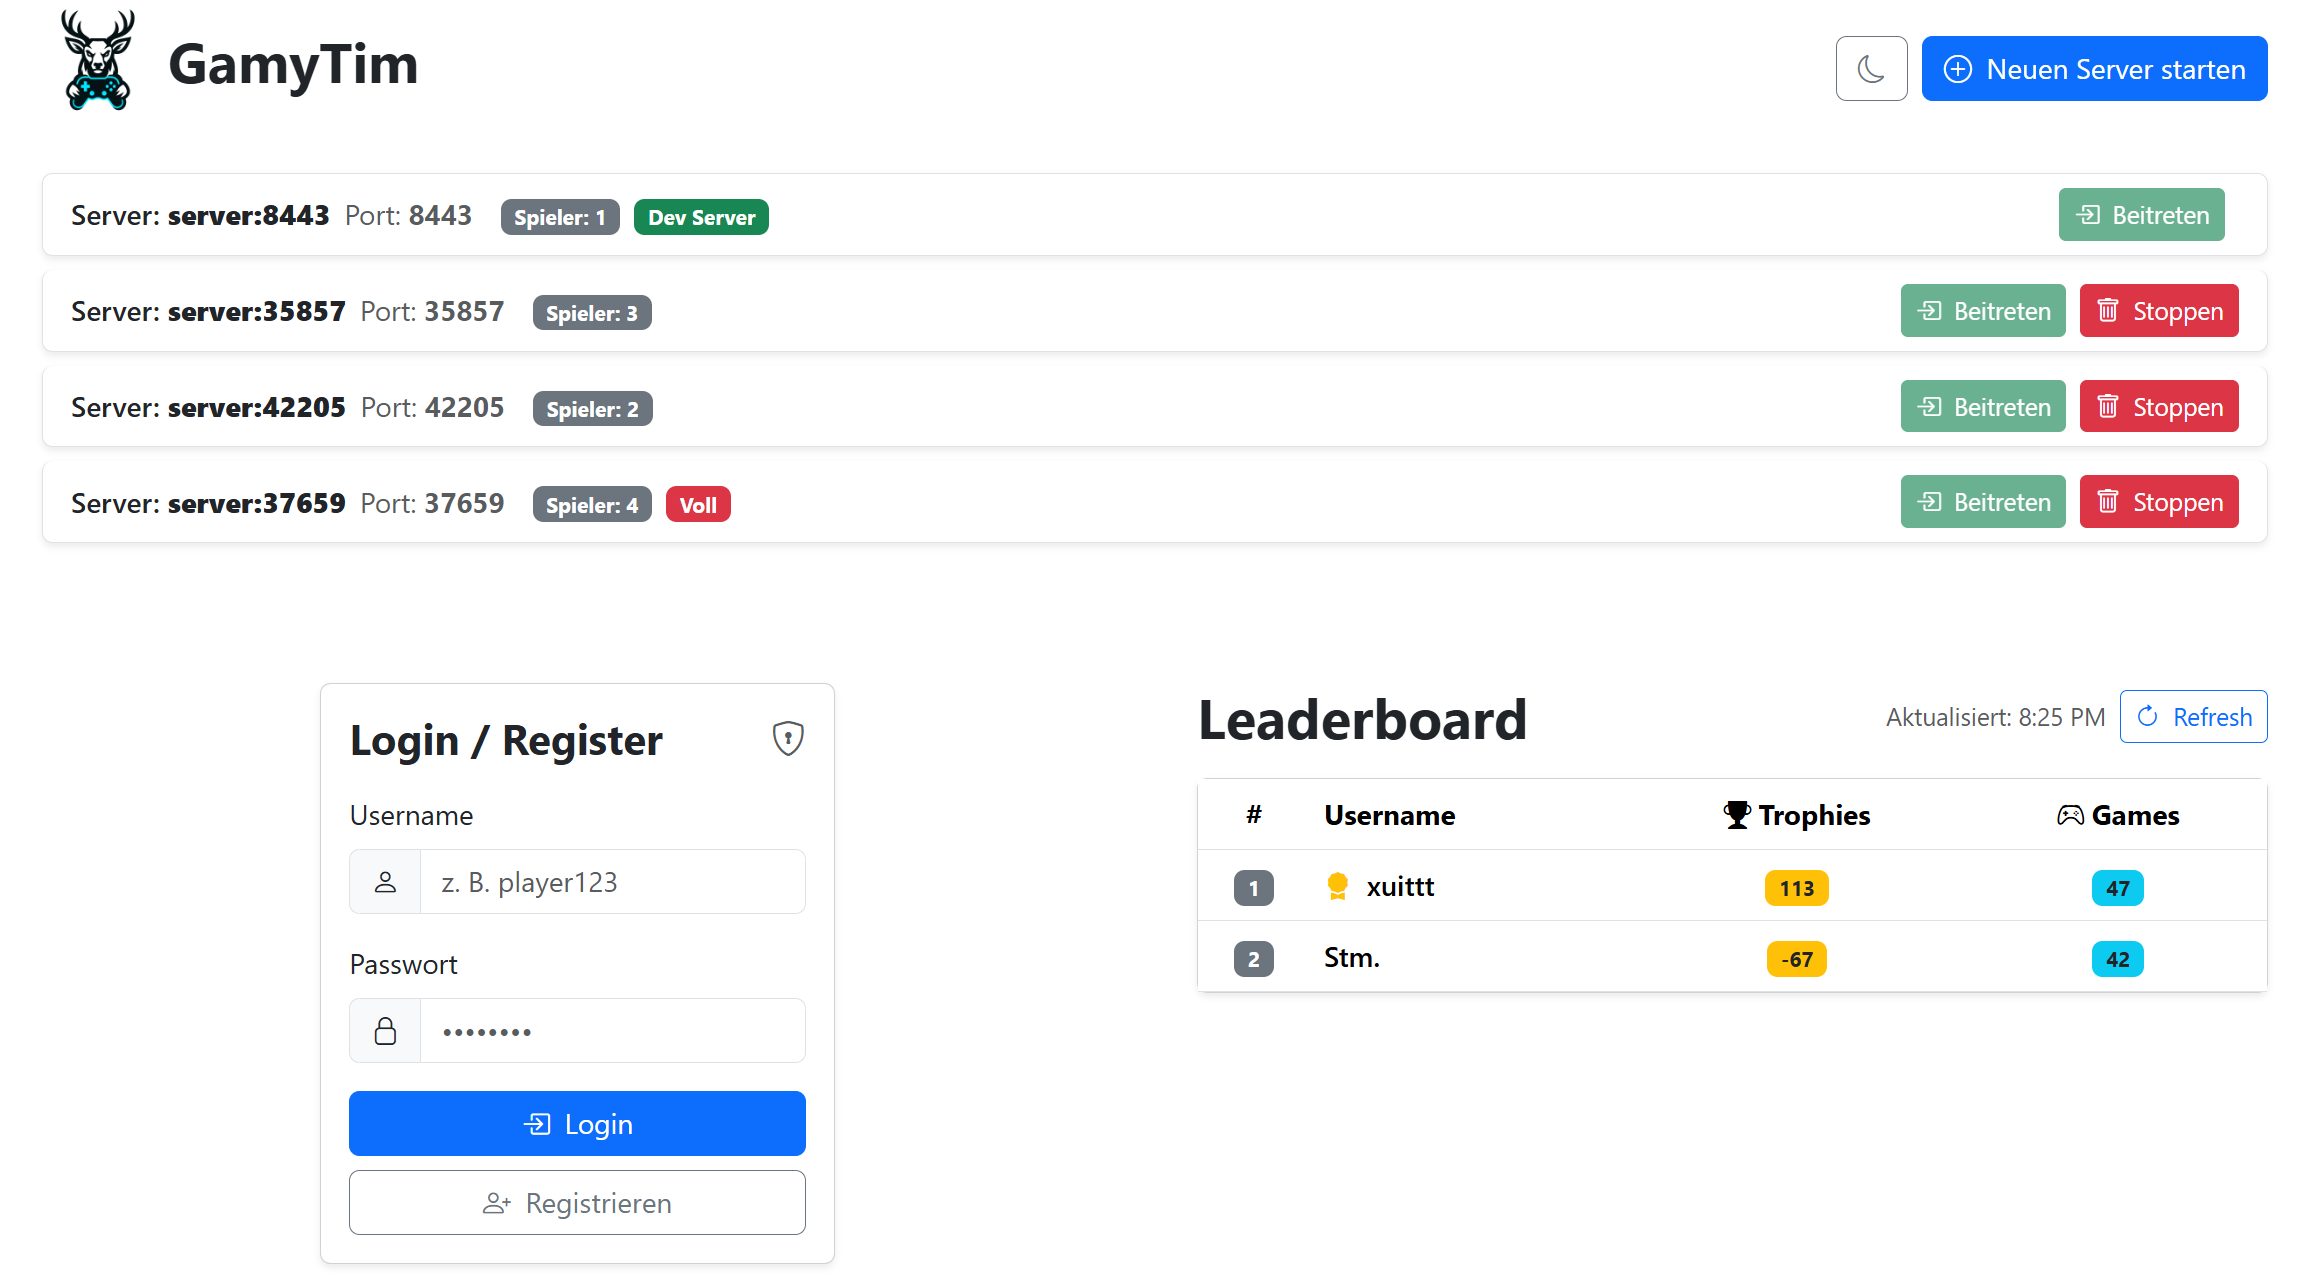
\includegraphics[width=1\linewidth]{../images/LobbyW.png}
  \caption{Frontend-Lobby des Projekts}
  \label{fig:frontend_lobby}
\end{figure}

\section{Funktionen der Lobby}
Die Frontend-Lobby umfasst mehrere Kernfunktionen, die jeweils mit Backend-Komponenten verknüpft sind:

\subsection{Login / Registrierung}
Über das Login-Formular können sich Benutzer mit einem bestehenden Account anmelden oder einen neuen Benutzer registrieren.  
Die Eingaben werden an die \textbf{UserDB} weitergeleitet, wo Validierung und Speicherung der Daten erfolgen.  
Nach erfolgreicher Anmeldung stehen dem Benutzer alle Funktionen der Lobby zur Verfügung.
\subsection{Token basierte Authentifizierung}*
Im Projekt wird die Authentifizierung über JWT umgesetzt.
Benutzer registrieren sich oder loggen sich ein, Passwörter werden mit bcrypt gehasht gespeichert.
Nach erfolgreichem Login erhält der Client ein Token, das bei allen Anfragen im Header mitgeschickt und vom Backend validiert wird.
Dadurch wird die Integrität der Benutzer-, Spiel- und Trophäendaten gewährleistet.
Um sich im GodotSpiel zu authentifizieren, wird das Token im URL-Parameter \texttt{token} übergeben, wodurch sicher gestellt wird, dass in Godot immer der Name sowie die Authorität des Spieler bekannt sind.
\noindent
Vgl. hierzu auch:  
Fettke, Peter; Vogel-Heuser, Birgit (Hrsg.): \textit{Digitale Authentifizierung und Autorisierung}, Springer Vieweg, 2021.  
Jones, M. et al.: \textit{JSON Web Token (JWT)}, IETF RFC 7519,May 2015. \url{https://datatracker.ietf.org/doc/html/rfc7519} (lezter Zugriff: 17.09.2025)

\subsection{Serverübersicht}
Im oberen Bereich wird die aktuelle Serververbindung angezeigt. 
Dabei sind \texttt{Servername}, \texttt{Port} sowie die Anzahl der verbundenen Spieler sichtbar.  
Die Daten stammen vom \textbf{Masterserver}, der kontinuierlich den Status aller verfügbaren Lobbys aktualisiert.

\subsection{Serververwaltung}
Benutzer können neue Serverinstanzen über den Button \glqq Neuen Server starten\grqq{} anlegen und ggf. bestehende Server über \glqq Stoppen\grqq{} wieder beenden.
Diese Anfrage wird an den \textbf{Loadbalancer} übermittelt, welcher die Instanz erstellt und die notwendigen Metadaten (z.\,B. Port, Lobby-ID) an den Masterserver weitergibt.

\subsection{Lobbybeitritt}
Mit der Funktion \glqq Beitreten\grqq{} können Spieler einer vorhandenen Lobby beitreten.  
Hierbei wird die Verbindung zu einem \textbf{Game-Server} hergestellt, der die eigentliche Spiellogik ausführt.  

\subsection{Leaderboard}
Das Leaderboard zeigt die globalen Punktestände und Spielstatistiken aller Spieler an.  
Die Daten werden aus der Datenbank geladen und im Frontend aktualisiert.  
Dargestellt werden unter anderem:
\begin{itemize}
  \item Benutzername,
  \item Anzahl der Trophäen,
  \item Anzahl gespielter Spiele.
  \item Leader
\end{itemize}
\subsection{Datenintegritäts-Sicherung}*
Im Backend wird über eine Validierung der einkommenden Trophäen- und Gamedaten die Integrität der Daten im Rahmen des Projektes angegangen.



\section{Godot-Spiel}
\label{chap:godot}

Das Spiel folgt dem klassischen Prinzip von \textit{Achtung, Kurve!}:  
Jeder Spieler steuert eine farbige Linie, die sich kontinuierlich über das Spielfeld bewegt.  
Ziel ist es, möglichst lange zu überleben, indem man nicht mit den Linien anderer Spieler oder den Spielfeldrändern kollidiert.  
Die Steuerung erfolgt ausschließlich über Richtungsänderungen (links/rechts).

\section{Spieloberfläche}
Die Spieloberfläche zeigt die farbigen Linien der aktiven Spieler sowie deren aktuelle Positionen (Abbildung~\ref{fig:godot_game}).  
Am oberen Rand werden die Punktestände der Spieler angezeigt, welche bei Kollisionen entsprechend angepasst werden.


\begin{figure}[h!]
  \centering
  
\includegraphics[width=1\linewidth]{../images/game.png}
  \caption{Spielfeld in Godot mit drei aktiven Spielern}
  \label{fig:godot_game}
\end{figure}
 
\newpage
\section{Lobby- und Ready-System}
Vor Spielbeginn wird eine Lobby-Ansicht geladen, in der sich alle Spieler sammeln.  
Hierbei übernimmt der erste Spieler die Rolle des \textbf{Hosts}.  
Alle weiteren Spieler treten über die Lobby bei.  
Jeder Spieler muss seinen Status auf \textit{Ready} setzen, bevor das Spiel starten kann.  
Die Synchronisation erfolgt über den Game-Server, der den Status aller Spieler an die Lobby zurückmeldet (Abbildung~\ref{fig:ready_system}).

\begin{figure}[h!]
  \centering
  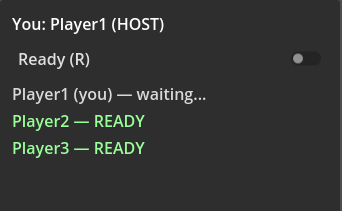
\includegraphics[width=0.4\linewidth]{../images/ready.png}
  \caption{Ready-System: alle Spieler müssen bereit sein, bevor das Spiel startet}
  \label{fig:ready_system}
\end{figure}

\noindent
Vgl. hierzu auch:  
Godot Engine Documentation: \textit{High-level multiplayer} und \textit{Networking fundamentals},  
\url{https://docs.godotengine.org/en/stable/tutorials/networking/high_level_multiplayer.html} (lezter Zugriff: 17.09.2025).  


\section{Synchronisation und Kommunikation}
Die Game-Server sind für die Synchronisation der Spiellogik verantwortlich.  
Dabei werden folgende Informationen zwischen den Instanzen ausgetauscht:
\begin{itemize}
  \item Spielerpositionen und Bewegungsrichtungen,
  \item Statusänderungen (z.\,B. Ready/Not Ready, Spielstart, Spielende),
  \item Kollisionsereignisse und daraus resultierende Punktestände.
\end{itemize}

Der zuvor bei Lobby-Beitritt festgelegte Host übernimmt die Rolle des \textbf{Master-Clients} und koordiniert die Spielabläufe.
D.h. wenn eine Kollision durch abweichende Spielabläufe auf Clientseite fälschlicherweise stattfinden, wird diese nicht erkannt. 
Nur Kollisionsereignisse, die der Master-Client erkennt, werden an alle Clients weitergegeben und somit erkannt. Dies führt zu einem geregelten Spielablauf.
Ein solches Verhalten (d.h. dass nur der Master-Client Kollisionsereignisse erkennt und propagiert) entspricht bekannten Entwurfsmustern in Multiplayer-Spielen, in denen eine autoritative Instanz (Server oder Host) nötig ist, 
um Inkonsistenzen durch etwaige Abweichungen in Client Simulationen zu vermeiden (vgl. z. B. Liljekvist, Detecting Synchronisation Problems in Networked Lockstep Games, KTH 2016; oder Artikel zu Netzwerk-Synchronisation in Multiplayer Games (lezter Zugriff: 17.09.2025) ).
	% Anhang
	\clearpage
	\pagenumbering{roman}

	% Abbildungsverzeichnis
	%\cleardoublepage
	%\phantomsection \label{listoffig}
	%\addcontentsline{toc}{chapter}{Abbildungsverzeichnis}
	%\listoffigures

	%Tabellenverzeichnis
	%\cleardoublepage
	%\phantomsection \label{listoftab}
	%\addcontentsline{toc}{chapter}{Tabellenverzeichnis}
	%\listoftables

	% Quellcodeverzeichnis
	%\cleardoublepage
	%\phantomsection \label{listoflist}
	%\addcontentsline{toc}{chapter}{Listings}
	%\lstlistoflistings

	% Literaturverzeichnis
	\cleardoublepage
	\phantomsection \label{listoflit}
	\addcontentsline{toc}{chapter}{Literaturverzeichnis}
	
	%Bib style
	\bibliographystyle{agsm} %Havard
	%\bibliographystyle{amsplain} %Durchnummeriert
	%\bibliographystyle{amsalpha} %Kürzel für Autor und Jahr
	%see more: http://amath.colorado.edu/documentation/LaTeX/reference/faq/bibstyles.pdf
	
	\bibliography{ArbeitBib}

	% Abkürzungsverzeichnis
	%\cleardoublepage
	%\phantomsection \label{listofacs}
	%\addcontentsline{toc}{chapter}{Abkürzungsverzeichnis}
	%%!TEX root = ../dokumentation.tex

\chapter*{Abkürzungsverzeichnis}
%nur verwendete Akronyme werden letztlich im Dokument angezeigt
\begin{acronym}[YTMMM]
\setlength{\itemsep}{-\parsep}

\acro{AGPL}{Affero GNU General Public License}
\acro{API}{Application Programming Interface}
\acro{WYSIWYG}{What You See Is What You Get}
\end{acronym}

	
	% Glossar
	%\printglossary[style=altlist,title=Glossar]
\end{document}
